\documentclass{amsart}
\title{Attacks on search-RLWE}
\author{Hao Chen, Kristin Lauter, Katherine E. Stange}

\usepackage{macros}
\usepackage{float}
\usepackage{url}
\usepackage{placeins}
\usepackage{hyperref}

\usepackage{algpseudocode}
%\usepackage{algorithmic}
\usepackage{algorithm}
\usepackage{physics}

\begin{document}
\maketitle

\begin{abstract}
We describe a new attack on the Ring learning-with-errors (RLWE) problem based on the chi-square statistical test, and give examples of Galois number fields vulnerable to our attack. We then analyze the security of cyclotomic fields against our attack.

%Also, we sharpen the attack in \cite{elos2015weak} and give examples of vulnerable instnaces of cryptographic size. Finally, we discuss the effect of modulus switching on our attacks.
\end{abstract}

\section{Introduction}
The Ring learning-with-errors (RLWE) problem, proposed in \cite{lyubashevsky2013ideal}, is a variant of the traditional learning-with-error (LWE) problem, and is an active research area in lattice based cryptography. It has been studied extensively in (a lot of papers).

Central to an RLWE problem instance is a choice of a number field $K$ and a prime $q$ called the {\it modulus}. The authors of \cite{lyubashevsky2013ideal} considered the case where $K$ is some cyclotomic field, and proved a reduction from certain hard lattice problems to the dual variant of RLWE. The hardness for the non-dual variant was proved in \cite{ducas2012ring}. Also in \cite{lyubashevsky2013ideal}, a search-to-decision reduction was proved for RLWE problems for cyclotomic fields and modulus $q$ which splits completely. This reduction was then generalized to general Galois extensions in \cite{eisentrager2014weak}.

The authors of \cite{elos2015weak} proposed an attack to decision RLWE problem. The attack makes use of ring homomorphisms $\pi: R \to \bF_q$, and works when the image of the RLWE error distribution under the map $\pi$ only takes value in a stricly smaller subset of $\bF_q$, with overwhelming probability. The authors of \cite{elos2015weak} then gave an infinite family of examples vulnerable to the attack. Unfortunately, the vulnerable number fields in \cite{elos2015weak} are not Galois extensions of $\bQ$. Hence, the search-to-decision reduction theorem does not apply, and the attack can not be directly used to solve the search variant of RLWE for those instances.

In our paper, we generalize the attack of \cite{elos2015weak} to Galois number fields and moduli of higher degree. Also, we analyze the vulnerability of cyclotomic fields to the \cite{elos2015weak} attack, and show that they are in general safe, except for the case when the modulus $p$ is equal to the index of the cyclotomic field (i.e., $K = \bQ(\zeta_p)$).


\subsection{Organization}

In section \ref{sec: background}, we recall the canonical embedding of number fields and the central definitions related to the RLWE problems. In section \ref{sec: s-to-d}, we review prime factorizations in Galois extensions and prove a search-to-decision reduction for Galois extensions $K$ and unramified primes of any degree. In section \ref{sec: chi-square}, we introduce an attack to RLWE problems based on the chi-square statistical test, which directly generalizes the attack in \cite{elos2015weak}. More precisely, the attack aims at two problems: the decision version of RLWE, and an intermediate problem used in the search-to-decision proof of \cite{lyubashevsky2013ideal}, which we denote by $\SRLWE(\cR,\fq)$ (see Definition~\ref{def: srlwe mod q}). The time complexity of our attack for both problems above is $O(\frac{n}{f}q^{2f})$, Here $n$ is the degree of the number field $K$, and $f$ is the {\it residual degree} of $q$ in $K$ (see Lemma~\ref{lem: prime factorization}). In section \ref{sec: sub-cyclotomics}, we give examples of subfields of cyclotomic fields vunlerable to our new attack, where the moduli $q$ has residual degree two.

In section \ref{sec: ramified-prime}, we show that our attack works on prime cyclotomic fields when the moduli is equal to the unique ramified prime. Finally, in section \ref{sec: cyclo-secure}, we show that general cyclotomic extensions with an unramified prime as the modulus $q$ are invulnerable to our attack.





\section{Background} \label{sec: background}

Let $K$ be a number field of degree $n$ with ring of integers $R$ and let $\sigma_1, \cdots, \sigma_n$ be the embeddings of $K$ into $\bC$, the field of complex numbers. The {\it canonical embedding} of $K$ is
\begin{align*}
    \iota: K &\to \bC^n \\
     x & \mapsto (\sigma_1(x), \cdots, \sigma_n(x)).
\end{align*}

To work with real vector spaces, we define the {\it adjusted embedding} of $K$ as follows. Let $r_1$, $r_2$ denote the number of real embeddings and conjugate pairs of complex embeddings of $K$. Without loss of generality, assume $\sigma_1, \cdots, \sigma_{r_1}$ are the real embeddings and $\sigma_{r_1+r_2+j} = \overline{\sigma_{r_1 + j}}$ for $1 \leq j \leq r_2$. We define

\begin{align*}
    \tilde{\iota}: K & \to \bR^n \\
    x & \mapsto (\sigma_1(x), \cdots, \sigma_{r_1}(x), \Re(\sigma_{r_1+1})(x), \Im(\sigma_{r_1+1})(x), \cdots,  \Re(\sigma_{r_1+r_2})(x), \Im(\sigma_{r_1+r_2})(x)).
\end{align*}

It turns out that $\tilde{\iota}(R)$ is a lattice in $\bR^n$. Let $w = (w_1, \cdots , w_n)$ be an integral basis for $R$.

\begin{Definition}
The canonical (resp. adjusted) embedding matrix of $w$, denoted by $A_w$ (resp. $\tilde{A_w}$), is the $n$-by-$n$ matrix whose $i$-th column is $\iota(w_i)$ (resp. $\tilde{\iota}(w_i)$).
\end{Definition}

The two embedding matrices are related in a simple way:
let $T$ denote the matrix
\[
T = \begin{bmatrix}
    I_{r_1}  & 0  \\
    0     & T_{r_2} \\
\end{bmatrix},
\mbox{ where } T_s = \frac{1}{\sqrt{2}} \begin{bmatrix}
    I_{r_2}  & I_{r_2} \\
    -iI_{r_2}     & iI_{r_2} \\
\end{bmatrix},
\]
Then we have
$$\tilde{A_{w}} = T A_{w},$$
and the lattice $\tilde{\iota}(R)$ has a basis consisting of columns of $\tilde{A_{w}}$.

For $\sigma > 0$, define the Gaussian function $\rho_\sigma: \bR^n \to [0,1]$ as $\rho_\sigma(x) = e^{-||x||^2/2\sigma^2}$ (our $\sigma$ is equal to $r/\sqrt{2\pi}$ for the parameter $r$ in \cite{lyubashevsky2013ideal}).
\begin{Definition}
For a lattiace $\Lambda \subset \bR^n$ and $\sigma > 0$, the {\it discrete Gaussian distribution} on $\Lambda$ with parameter $\sigma$ is:
\[
    D_{\Lambda, \sigma}(x) = \frac{\rho_\sigma(x)}{\sum_{y \in\Lambda} \rho_\sigma(y)}, \, \forall x \in \Lambda.
\]
\end{Definition}
Equivalently, the probability of sampling any lattice point $x$ is proportional to $\rho_\sigma(x)$.

\subsection{Ring LWE problems for general number fields}

\begin{Definition}
An {\it RLWE instance} is a tuple $\cR = (K,q,\sigma,s)$, where $K$ is a number field with ring of integers $R$, $q$ is a prime, $\sigma >0$, and $s \in R/qR$ is the {\it secret}.
\end{Definition}


\begin{Definition}
Let $\cR = (K,q,\sigma,s)$ be an RLWE instance and let $R$ be the ring of integers of $K$. The {\it error distribution} of $\cR$, denote by $D_\cR$, is the discrete lattice Gaussian distribution
\[
D_\cR = D_{\tilde{\iota}(R),\sigma}.
\]
\end{Definition}

Let $n$ denote the degree of $K$. As is pointed out in \cite{elos2015weak}, when analyzing the error distribution, one needs to take into account the sparsity of the lattice $\tilde{\iota}(R)$, which is measured by its covolume $V_R$. In light of this, we define a relative version of the standard deviation parameter: $$\sigma_0 = \frac{\sigma}{V_R^{\frac{1}{n}}}.$$

\begin{Definition}[RLWE distribtuion]
Let $\cR = (K,q,\sigma, s)$ be an RLWE instance with error distribution $D_\cR$, We let $R_q$ denote $R/qR$, then
a sample from the {\it RLWE distribtuion} of $\cR$ is a tuple
$$(a, b = as+e\pmod{qR}) \in R_q \times R_q, $$
where the first coordiante $a$ is chosen uniformly at random in $R_q$, and $e \gets D_\cR$.
\end{Definition}

We use the shorthand notation $(a,b) \gets \cR$ to represent that $(a,b)$ is sampled from the RLWE dsitribution of $\cR$. The RLWE problem has two major variants: search and decision.

\begin{Definition}[Search]
Let $\cR$ be an RLWE intance. The {\it search Ring-LWE} problem, denoted by $\SRLWE(\cR)$, is to discover $s$ given access to arbitrarily many independent samples $(a,b) \gets \cR$.
\end{Definition}

\begin{Definition}[Decision]
Let $\cR$ be an RLWE intance. The {\it decision Ring-LWE}
problem, denoted by $\DRLWE(\cR)$, is to distinguish between the same number of independent samples in two distributions on $R_q \times R_q$. The first is the RLWE distribution of $\cR$, and the second consists of uniformly random and independent samples from $R_q \times R_q$.
\end{Definition}

\subsection{Sampling methods}
In practice, there are different ways to approximately sample from the RLWE error distribution $D_\cR$, and we will switch between three sampling methods in our paper. While searching for weak Galois RLWE instances, we use the sampling algorithm in  \cite{gentry2008trapdoors}; when analyzing the security of cyclotomics, we defined a modified error distribution $MD_{m,q,k}$ (see Definition~\ref{def: modified distribution}); when proving the vulnerability of prime cyclotomics at the ramified prime, we used the PLWE sampling method, which samples each coefficient of the error polynomial independently from a discrete Gaussian over the integers. We mention that \cite{lyubashevsky2013toolkit} has an efficient algorithm for cyclotomic fields. Since it is primarily related to the dual version of RLWE, we will not use it in our paper.


\section{search-to-decision reduction}
\label{sec: s-to-d}

The main result of this section (Corollary~\ref{cor: s-to-d}) is a reduction from SRLWE to DRLWE for Galois fields $K$ and unramified primes $q$. We will prove the reduction from SRLWE to an intermediate problem, which we denote by $\SRLWE(\cR,\fq)$ (it is denoted by $\fq_i$-LWE in \cite{lyubashevsky2013ideal}). This result can be viewed as a generalization of \cite[Theorem 2]{eisentrager2014weak} to primes of higher degree. Since our attack in Section~\ref{sec: chisquare} is  targeting at $\SRLWE(\cR,\fq)$, we could attack SRLWE for any Galois RLWE instances vulnerable to our attack.

%We remark that a search-to-decision reduction theorem for higher degree primes can be proved by carrying out almost the exact same proof in \cite{eisentrager2014weak}.

\begin{Definition} \label{def: srlwe mod q}
Given an RLWE instance $\cR = (K,q,\sigma, s)$ and a prime ideal $\fq$ of $K$ lying above $q$. The problem $\SRLWE(\cR, \fq)$ is: given access to arbitrarily many independent samples $(a,b) \gets \cR$, find $s \pmod {\fq}$.
\end{Definition}

We recall some facts from algebraic number theory in the following lemma.
\begin{Lemma}
\label{lem: prime factorization}
Let $K/\bQ$ be a finite Galois extension with ring of integers $R$,  and let $q$ be a prime unramified in $K$. Then there exists an integer $g \mid n$, and a set of $g$ distinct prime ideals $\fq_1, \cdots ,\fq_g$ of
$R$ such that
\[
    qR = \prod_{i=1}^g \fq_i.
\]
Let $f = \frac{n}{g}$. Then the quotient $R/\fq_{i}$ is a finite field of cardinality $q^f$  for each $i$. There is a canonical isomorphism of rings
\[
    R_q \cong R/\fq_{1} \times \cdots \times R/\fq_{g}.
\]
\end{Lemma}
The number $f$ in the above lemma is called the {\it residual degree} of $q$ in $K$. Note that the prime $q$ splits completely in $K$ if and only if its residual degree is one.


\begin{theorem} \label{thm: reduction}
Let $\cR = (K,q,\sigma, s)$ be an RLWE instance with $K/\bQ$ Galois and $q$ unramified in $K$ with residual degree f. Suppose there is an algorithm $\sA$ which solves $\SRLWE(\cR,\fq)$ using a list $S$ of samples. Assume that the running time of the algorithm $\sA$ is $t$. Then the problem $\SRLWE(\cR)$ can be solved in time $T = \frac{n}{f}t$ using the samples in $S$.
\end{theorem}

\begin{proof}
The Galois group $G =Gal(K/\bQ)$ acts on the set $\{\fq_1, \cdots ,\fq_g\}$ transitively. Hence for each $i$, we can take $\sigma \in Gal(K/\bQ)$, such that $\sigma_i(\fq) = \fq_i$, Then we run the algorithm $\sA$ on the input $(\sigma_i^{-1}(S), \fq_i)$. The algorithm will output $\sigma_i^{-1}(s) \pmod{\fq}$, which is equal to $s \pmod{\fq_i}$. We then do this for all $1\leq i \leq g$ and use the last formula of Lemma to recover $s$. The complexity estimate follows from the fact that we are applying the algorithm $g$ times.
\end{proof}

Theorem~\ref{thm: reduction} gives a polynomial time reduction from $\SRLWE(\cR)$ to $\SRLWE(\cR,\fq)$.

\begin{remark}
Note that in the complexity computation above we have chosen to neglect the time taken by applying Galois automorphisms to the samples, because the runtime depends
hugely on the instance and on the way we represent the samples. For example, for subfields of cyclotomic fields with normal integral bases, the Galois autormophisms are simply permutations of coordinates, so the time needed to apply these automorphisms is trivial.
\end{remark}

%\begin{remark}
%Although the theorem is stated for any unramified prime. From an %attacker's perspective, we still take primes of small degree, since the search space for $s \pmod{\fq}$ is of size $q^f$, and it is bad when $f$ is large.
%\end{remark}

The search-to-decision reduction will follow from the lemma below.
\begin{Lemma}
There is a probablistic polynomial time reduction from $\SRLWE(\cR,\fq)$ to $\DRLWE(\cR)$.
\end{Lemma}

\begin{proof}
This is a rephrasing of \cite[Lemma 5.9 and Lemma 5.12 ]{lyubashevsky2013ideal}.
\end{proof}

\begin{Corollary}\label{cor: s-to-d}
Suppose $\cR$ is an RLWE instance where $K$ is Galois and $q$ is an unramified prime in $K$. Then there is a probablistic polynomial-time reduction from $\SRLWE(\cR)$ to $\DRLWE(\cR)$.
\end{Corollary}

\section{The chi-square attack for uniform distribution}
\label{sec: chi-square}
\subsection{chi-square test for uniform distribution}
We briefly review the properties and usage of the chi-square test for uniform distributions over a finite set $S$. We partition $S$ into $r$ subsets $S = \bigsqcup_{j=1}^r S_i$.
Suppose there are $M$ samples $y_1, \cdots, y_M \in S$.
For each $1 \leq j \leq r$, we compute the expected number of samples that would fall in the $j$-th subset: $c_j := \frac{|S_j|M}{|S|}$. Then we compute the actual number of samples in $S_j$, i.e., $t_j := |\{1 \leq i \leq r: y_i \in S_j\}|$. Finally, the $\chi^2$ value is computed as
\[
    \chi^2(S,y) = \sum_{j = 1}^r \frac{(t_j -c_j)^2}{c_j}.
\]
Suppose the samples are drawn from the uniform distribution on $S$. Then the $\chi^2$ value follows the chi-square distribution with degree of freedom equal $d = r-1$.
To decide whether the samples are from a uniform distribtuion, we can either look up a table of $\chi^2$ values, or use an approximation rule:  when $d$ is large, the $\chi^2$ distribution can be well-approximated by a normal distribution $N(d, 2d)$.

If $P,Q$ are two probability distributions on the set $S$, then their {\it statistical difference} is defined as
\[
    d(P,Q) = \frac{1}{2} \sum_{t \in S} |P(t) - Q(t)|.
\]
For convenience, we also define the {\it $l_2$ distance} between $P$ and $Q$ as $d_2(P,Q) = (\sum_{t \in S} |P(t) - Q(t)|^2)^{\frac{1}{2}}$. We have the inequality $d(P,Q) \leq \frac{\sqrt{|S|}}{2}d_2(P,Q)$.



\subsection{The chi-square attack on $\SRLWE(\cR,\fq)$}

Let $\cR$ be an RLWE instance with error distribution $D_{\cR}$ and $\fq$ be a prime ideal above $q$.  The basic idea of our attack relies on the assumption that the distribution $D_\cR \pmod {\fq}$ is distinguishable from the uniform distribution on the finite field $F = R/\fq$. More precisely, the attack loops through all $q^f$ possitbilities of $\bar{s} = s \pmod{\fq}$, and for each guess $s'$, it computes the values $\bar{e}' = \bar{b} - \bar{a} s' \pmod {\fq}$ for every sample $(a,b) \in S$. If the guess is wrong, or if the samples are taken from the uniform distirbution in $(R_q)^2$, the values $\bar{e}'$ would be uniformly distributed in $F$ and it is likely to pass the chi-square test. On the other hand, if the guess is correct, then we expect the test on the errors $\bar{e}'$ to reject the null hypothesis.

Let $N = q^f$,  the cardinality of $F$. For the attack to be successful, we need the $(N-1)$ tests corresponding to wrong guess of $s \pmod{\fq}$ to pass, and the one test corresponding to the correct guess to be rejected. For example, we may choose the confidence level to be  $\alpha = 1 - \frac{1}{10N}$. The detailed attack is described in Algorithm~\ref{alg: chi-square}. Note that the time complexity of the attack is $O(N)$ since there are $N$ possible values for $s \pmod {\fq}$. The number of samples need for the attack is also $O(N)$, as required by the chi-square test.
%Let $\beta$ denote the probability that the sample errors fails the uniform test with probability  Then the probability that our algorithm will success is $p  = (1- \frac{1}{10N})^{N-1} \beta$. Note that when $N$ is large, $(1- \frac{1}{10N})^{N-1}$ is about $e^{-1/10} \approx 0.904$.


%Note that although we restrict ourselves to subfields of cyclotomics with odd and square-free $m$, the attack could be applied to any finite extension of $\bQ$.

\begin{algorithm}[H] \label{alg: chi-square}
\caption{chi-square attack of $SRLWE(\cR,\fq$)}          % give the algorithm a caption
\label{IPR}                           % and a label for \ref{} commands later in the document
\begin{algorithmic}[1]              % enter the algorithmic environment
     \Require

     %$A_{\bf a}$: the embedding matrix, where ${\bf a}$ is a basis for the ring of integers $\cO_K$ of some number field $K/\bQ$.
     $\cR = (K,q,\sigma, s)$ -- an RLWE instance; $R$ -- the ring of integers of $K$; $\fq$ -- a prime ideal in $K$ above $q$; $B$ -- the number of bins ($B \leq |F|$); $\mathcal{S}$ -- a collection of $M$ ($M = \Omega(|F|)$) RLWE samples from $\cR$.
    \Ensure a guess of the value $s \pmod{\fq}$, or {\bf NON-RLWE}, or {\bf INSUFFIICNET-SAMPLES}

    \State $\omega \gets \Phi^{-1}(1- \frac{1}{20N})$, $\cG \gets \emptyset$

    \For{$s$ in $F$}
        \State $\cE \gets \emptyset$.
        \For{$a,b$ in $\mathcal{S}$}
            \State $\bar{a}, \bar{b} \gets a \pmod{\fq}, b \pmod{\fq}$.
            \State $\bar{e} \gets \bar{b} - \bar{a}s$.
            \State add $\bar{e}$ to $\cE$.
        \EndFor

        \State Run $\chi^2$ test on the set $\cE$ and $B$ bins to obtain the value $\chi^2(\cE)$.
        \If{$|\chi^2(\cE) - (B-1)| > \omega \sqrt{2B-2}$}
            \State add $s$ to $\cG$.
        \EndIf
    \EndFor
    \If{$G = \emptyset$}

        \Return {\bf NOT RLWE}
    \ElsIf{$G = \{g\}$}

        \Return $g$
    \Else
        \Return {\bf INSUFFIICNET-SAMPLES}
    \EndIf

\end{algorithmic}
\end{algorithm}



The correctness of the attack is captured in Theorem~\ref{thm: attack}. We use $D_{\cR,\fq}$ as a shorthand notation for $D_{\cR} \pmod{\fq}$.  Let $\Phi$ denote the cumulative distribution function of the standard Gaussian distribution.

\begin{theorem} \label{thm: attack}
Let $\Delta$ denote the statistical distance between the distribution $D_{\cR, \fq}$ and the uniform distribtuion on $R/\fq$. Let $\lambda = 4 M \Delta^2$ and $\omega = \Phi^{-1}(1- \frac{1}{20N})$. Finally, let $p$ denote the proability of success of the attack in Algorithm~\ref{alg: chi-square}. When $q \gg 1$, we have

$$p  \geq 0.904 \left(1- \Phi \left(\frac{\omega \sqrt{2(N-1)}- \lambda}{\sqrt{2(N-1) +4\lambda}}\right) \right) - o(1).$$
\end{theorem}

\begin{proof}
It is a standard fact that chi-square value on samples from $D_{\cR, \fq}$, when the null hypothesis is uniform, follows a non-central chi-square distribution with the same degree of freedom and a parameter $\lambda_0$ given by
\[
    \lambda_0 =  d_2(D_{\cR, \fq}, U(R/\fq))^2 \cdot MN.
\]
In particular, we have $\lambda_0 \geq  4M\Delta^2 = \lambda$. Since $q \gg 1$, we may approximate a noncentral chi-square distribution with degree of freedom $k$ and parameter $\lambda_0$ with a Gaussian distribution of mean $k + \lambda_0$ and variance $2k + 4\lambda_0$ (see \cite{ryabko2004new}, for example). Recall that our attack succeeds if the set $\cE$ from all $(N-1)$ wrong guesses passes the test, and the true errors modulo $\fq$ fail the test. The first event happens with probability $(1 - \frac{1}{10N})^{N-1} \geq e^{-1/10} = 0.904 \cdots$. The second event has probability $1 - \Phi \left(\frac{\omega \sqrt{2(N-1)}- \lambda_0}{\sqrt{2(N-1) +4\lambda_0}}\right) $, which is an increasing function in $\lambda_0$. The theorem now follows.
\end{proof}

\begin{remark}
One could vary $\omega$ in Theorem~\ref{thm: attack} to suit the specific instance.
The probability of success will change accordingly. When we expect the statistical distance $\Delta$ to be large, it is preferable to choose a larger $\omega$ to increase the probability of success.
\end{remark}

The following is a plot of $p$ versus $\Delta$ for various choices of $N$, made according to Theorem~\ref{thm: attack}, where we fix the number of samples to be $M = 5N$.

\begin{center}
\includegraphics[width = 0.60\textwidth]{attack-quality.png}
\end{center}

\section{Vulnerable instances among subfields of cyclotomic fields}\label{sec: sub-cyclotomics}

When searching for vulnerable instances to our attack, we restrict our attention to subfields of cyclotomic fields $\bQ(\zeta_m)$, where we assume $m$ is {\it odd and squarefree}. The Galois group $\Gal(\bQ(\zeta_m)/\bQ)$ is canonically isomorphic to $G = (\bZ/m\bZ)^*$. For each subgroup $H$ of $G$, let $K_{m,H} = \bQ(\zeta_m)^H$ be the subfield of elements fixed by $H$.
Then the extension $K_{m,H}/\bQ$ is Galois with degree $n = \frac{\varphi(m)}{|H|}$. Also, the degree of a prime $q$ in $K_{m,H}$ is equal to the order of $[q]$ in the quotient group $G/H$. Moreover, $K_{m,H}$ has canonical {\it normal integral basis}, whose embedding matrix is easy to compute. More precisely, let $C$ denote a set of coset representatives of the coset space $G/H$. For each $c \in C$, set
\[
    w_c =  \sum_{h \in H} \zeta_m^{hc}.
\]
Then  $w := (w_c)_{c \in C}$ is a $\bZ$-basis of $R$. (For a proof of this fact, see \cite[Proposition 6.1]{johnston2011notes}). Setting $\zeta = \exp(2\pi i /m)$, the canonical embedding embedding matrix of $w$ is
\[
    (A_w)_{i,j} = \sum_{h \in H}{\zeta^{hij}}.
\]

\begin{Lemma} \label{lem: symmetry}
Suppose $\cR$ is an RLWE instance such that the underlying field $K$ is a Galois number field and $q$ is unramified in $K$. Then the reduced error distribution $D_{\cR,\fq}$ is independent of the choice of prime ideal $\fq$ above $q$.
\end{Lemma}

\begin{proof}
From the proof of Theorem~\ref{thm: reduction}, we know that the change from a prime $\fq$ to $\fq'$ can be done via applying an element of the galois group $\Gal(K/\bQ)$ to the RLWE samples. On the other hand, the Galois group acts on the embedded lattice $\Lambda_R$ by permuting the coordinates. Hence we have a group homomorphism $$\phi: \Gal(K/\bQ) \to \Aut(\Lambda).$$ Since permutation matrices are orthogonal, the Galois group action on $\Lambda_R$ given by $\phi$ is distance-preserving. In particular, it preserves any discrete Gaussian distribution on $\Lambda_R$. This completes the proof.
\end{proof}

\subsection{Searching}

Algorithm~\ref{alg: chi-square} allows us to search for vulnerable instances among fields of form $K_{m,H}$ by generating actual RLWE samples and running the attack. Success of the attack will indicate vulnerability of the instance. Note that our field searching requires sampling efficiently from a discete Gaussian $D_{\Lambda, \sigma}$, for which we use the efficient algorithm of \cite{gentry2008trapdoors}.

In Table~\ref{tab: attacked}, we list some instances on which the attack has succeeded. The columns of Table~\ref{tab: attacked} are as follows. The first two columns specify $m$ and the generators of $H$; the column labeled $f$ is the residual degree of $q$. The last column consists of either the runtime for an actual attack, or an estimation of the runtime. Note that we omited our choice of prime ideal $\fq$, since due to Lemma~\ref{lem: symmetry} the choice of $\fq$ is irrelevant to our attack.

\begin{table}[H] \label{tab: attacked}
\caption{Attacked sub-cyclotomic RLWE instances}
\begin{tabular}{c|c|c|c|c|c|c|c}
$m$ & generators of $H$ & $n$ & $q$ & $f$ & $\sigma_0$ & no. samples & runtime (in hours) \\ \hline
2805 &  [1684, 1618] & 40 & 67 & 2 & 1 & 22445 & 3.49 \\
15015 & [12286, 2003, 11936] & 60 & 43 & 2 & 1 & 11094 & 1.05 \\
15015 & [12286, 2003, 11936] & 60 & 617 & 2 & 1.25 & 8000 & 228.41 (estimated) \footnotemark  \\
90321 & [90320, 18514, 43405] & 80 & 67 & 2 & 1 & 26934 & 4.81 \\
255255 &  [97943, 162436, 253826, 248711, 44318] & 90 & 2003 & 2 & 1.25 & 15000 &  1114.44 (estimated) \\
285285 & [181156, 210926, 87361] & 96 & 521  & 2 & 1.1 & 5000 & 75.41 (estimated) \\
1468005Z & [312016, 978671, 956572, 400366] & 100 & 683 & 2 & 1.1
& 5000 &  276.01 (estimated) \\
1468005 & [198892, 978671, 431521, 1083139] & 144 & 139 & 2 & 1 &  4000 &  5.72
\end{tabular}
\end{table}


\footnotetext{The ``estimated'' runtime means that we did not perform the full attack. Instead, we ran  several chi-square tests and estimate the runtime based on the average time for running one test.}


%More precisely, suppose $\widehat{\chi^2}$ is the chi-square value of the sample errors from $D_{\cR, \fq}$. We replace $\lambda$ by $\widehat{\chi^2}$ in the formula and compute
%%    \widehat{p}  = 0.904 \left(1 - \Phi \left(\frac{\Phi^{-1}(1- \frac{1}{20N})\sqrt{2(N-1)}- \widehat{\chi^2}}{\sqrt{2(N-1) +4\widehat{\chi^2}}}\right)\right).
%\]
%The value $\widehat{p}$ is then our estimate of the sucess rate of our attack.  In addition, we estimate the runtime based on the average time taken for the tests we've done.

\subsection{Discussion}
One may notice that in all the vulnerable instances in Table~\ref{tab: attacked}, the prime $q$ has degree $f = 2$ in $K$. We have found the reason behind this phenomenon. Let $K$  be a Galois number field and suppose $q$ is a prime of degree $r$ in $K$. Suppose we have found a reduced basis $w_1,\cdots, w_n$ of $R$ with respect to the adjusted embedding. Fix a prime ideal $\fq$ above $q$. Then the images of the basis under the reduction modulo $\fq$ map are elements of $F = R/\fq$. Now if for some index $i$, the element $w_i$ lies inside some proper subfield $K'$ of $K$, and if $q$ has residual degree $r' < r$ in $K'$, then $w_i \pmod{\fq}$ will lie in a proper subfield of $F$. If the above situation happens for a large amount of the basis elements $w_i$, then we could  expect the reduced error distribution $D_{\cR,\fq}$ to take values in a proper subfield of $F$ more frequently. This would allow us to distinguish it from the uniform distribution on $F$.

\subsection{A detailed example}
In order to illustrate our discussion above together with the search-to-decision reduction, we study a vulnerable Galois RLWE instance in detail, where we generated RLWE samples, performed the attack, and used search-to-decision reduction to recover the entire secret $s$.


Let $m = 3003$ and $H$ be the subgroup of $(\bZ/m\bZ)^*$ generated by 2276, 2729 and 1123. Then $K = K_{m,H}$ is a Galois number field of degree $n = 30$. After a LLL lattice reduction on the canonical basis $w$, we obtained an basis $v_1, \cdots, v_n$ for the ring of integers $R$, ordered by increasing embedding length. We take the moduli to be $q = 131$, a prime of degree two in $K$. Finally, we take $\sigma_0 = 1$ and generate the secret $s$ from the discrete Gaussian $D_{\Lambda_R, \sigma}$. It turns out that there are 15 prime ideals in $K$ lying above $q$, which we denote by $\fq_1, \cdots, \fq_{15}$. We choose a prime $\fq$ above $q$ and denote by $\bar{v}$ the image of $v$ in $R/\fq$. We use $\bF_q$ to denote the prime subfield of $R/\fq \cong \bF_q^2$. It turns out that $\bar{v_i} \in \bF_q$ for $1 \leq i \leq 15$. We generated 1000 RLWE samples and used Algorithm~\ref{alg: chi-square} and Theorem~\ref{thm: reduction} to recover $s \pmod {\fq_i}$ for each $1 \leq j \leq 15$. Then we used Chinese remainder theorem to recover $s$. The attack succeeded in 32.8 hours.





\section{Attacking prime cyclotomic fields when the modulus is the ramified prime}
\label{sec: ramified-prime}

\subsection{Attacking the ramified prime} Let $p$ be an odd prime and $K = \bQ(\zeta_p)$. Then $K$ has degree $(p-1)$ and discriminant $p^{p-2}$.
In addition, the prime $p$ is totally ramified in $K$. There is a unique prime ideal $\fp = (1 - \zeta_p)$ above $p$, and the reduction map  $\pi: R/pR \to \bF_p$ satisfies
\[
        \pi(\zeta_p^i) = 1, \quad \forall i \in \bZ.
\]
Writing an RLWE error as  $e = \sum e_i \zeta_m^i$, we have $e \pmod{\fp} = \sum_i e_i$. Since the coefficients $e_i$ tends to be small, it is conceivable that  $e \pmod{\fp}$ takes on small values with higher probability, making the instance vulnerable to our chi-square attack. Table~\ref{tab: ramified} contains some data of some actual attacks we have done.

\begin{table}[H]
\label{tab: ramified}
\caption{attacks on DRLWE for $K= \bQ(\zeta_p)$ and $q = p$}
\begin{tabular}{c|c|c}
$p$ & $\sigma_0$ & runtime(in seconds) \\
\hline
251 & 0.5 & 2.62\\
503 & 0.575 & 12.02\\
809 & 0.61 & 34.38\\
\end{tabular}
\end{table}











%The root determinant of the embedded lattice $\tilde{\iota}(R)$ is $p^{\frac{p-2}{2(p-1)}}$.

%Let $\sigma_0$ denote the relative standard deviation parameter. Then we set $\sigma  = \sigma_0 p^{\frac{p-2}{2(p-1)}}$. The RLWE problem being considered is $\cR = (R, p, \sigma_0, s)$.

%Note that for the above analysis, we did not take the actual RLWE error distribution; instead, we generate the errors by sampling the coefficient of each basis vector independently
%from a discrete Gaussian integer distribution. This method of sampling is used in a related problem usually referred to as Poly-LWE (PLWE). The PLWE and RLWE error distributions are different. However, we will show that for our attack on ramified primes, they behave the same.


%For the sake of simplicity, we choose a different error distribution for our RLWE problem, which is introduced by \cite{ducas2012ring}. Consider the elements $v_i = \zeta_p^{i}$ of $R$. Note that the first $v_0, \cdots, v_{p-2}$ form a basis for $R$, and we have the relation
%$v_{p-1} = -\sum_{i=0}^{p-2}(v_i)$. Sampling from the \cite{ducas2012ring} error distribution, which we denote by $DD_{p,\sigma}$, consists of three steps: first, we generate a vector $(g_0, \cdots, g_{p-1})$, where $g_i$ are i.i.d. random variables under the continuous Gaussian distribution $N(0,\sigma^2)$. Then we form the sum
%$\sum g_i \zeta_p^i$ and use the relation to rewrite it as $\sum_{i=0}^{p-2} (g_i - g_{p-1}) \zeta_p^i$.
%Finally, we take the nearest integer of each coordinates and the error is $$e  = \sum_{i=0}^{p-2} [g_i - g_{p-1}] \zeta_p^i.$$

%The authors of \cite{ducas2012ring} describe the relation between standard deviation parameters in their sampling and the one in RLWE. Their Lemma roughly says that $DD(p, \sigma)$ is a close approximation to $D_{\tilde{\iota}(\bZ[\zeta_p]),\sqrt{p}\sigma}$.

%Under some mild assumptions, we will show that $e \pmod {\fp}$ takes on a proper subset of $\bF_p$.
%First, let $\{g\} =  g - [g]$ denote the distance from a real number $g$ to its nearest integer.

%{\bf Assumption} Suppose $g \gets N(0,\sigma^2)$, we assume that $\{g\}$ is distributed uniformly in $[-1/2,1/2]$. Note that this assumption is reasonable as long as $\sigma$ is not too small, e.g., $\sigma >10$ will do.

%Then we prove
%\begin{Prop} \label{prop: ramified}
%Suppose $\sigma > 10$ and $e \gets DD_{p, \sigma}$. Then for all $w > \sqrt{p\sigma^2 + 4(p-1)/3}$, we have
%\[
%    \prob(|e\pmod{\fp}| > w) < 2 - 2\Phi^{-1}(\frac{w}{\sqrt{p\sigma^2 + 4(p-1)/3}}) + o(1).
%\]
%\end{Prop}

%\begin{proof}
%\begin{align*}
%e \pmod {\fp} &= \sum_{i=0}^{p-2} g_i - (p-1)g_{p-1} - \sum_{i=0}^{p-2} \{g_i - g_{p-1}\} \\
%& = \sum_{i=0}^{p-1} g_i - \sum_{i=0}^{p-2} \{g_i - g_{p-1}\}
%\end{align*}
%By definition of the $g_i$, we have $\sum_{i=0}^{p-1} g_i \sim N(0, p\sigma^2)$. By our assumption, $\{g_i - g_{p-1}\} \sim U(-1/2,1/2)$ for each index $i$, with variance $4/3$. By the central limit theorem, when $p$ is large enough the distribution of $\sum_{i=0}^{p-2} \{g_i - g_{p-1}\}$ is approximated by $N(0, 4(p-1)/3)$. Hence $e \pmod{\fp}$ can be well approximated by $N(0, \sigma')$, where $\sigma' = p\sigma^2 + 4(p-1)/3$. The claim now follows.
%\end{proof}

%\begin{Corollary}
%If $p$ is a sufficiently large prime and $\sigma = o(\sqrt{p})$, then the \cite{elos2015weak} attack works on the RLWE instance $\bQ(\zeta_p)$ with modulus $p$ and the error distribution $DD(p, \sigma)$.
%\end{Corollary}

%\begin{proof}
%The attack in \cite{elos2015weak} is guaranteed to work provided
%\[
 %   \frac{p}{|e \pmod{\fp}|} > 2,
%\]
%with overwhelming probability.
%Assuming $\sigma = o(\sqrt{p})$, then by Proposition~\ref{prop: ramified} (take $w = 20$, for example, so that the right hand side is negligibly small), we have $\frac{p}{|e \pmod{\fp}|} \to \infty$ when $p \to \infty$. This completes the proof.
%\end{proof}

%\begin{Lemma} \qquad \\
%(1) $A_v^t A_v = pI_{p-1} - {\bf 1} {\bf 1}^t$.\\
%(2) For all $x \in \bR^n$, $||x||_2 \leq ||A_v x||_2 \leq p||x||_2$. \\
%(3) For all $x \in \bR^n$, $||y||_2 \leq ||A_v x||_2 \leq %(3) $A_v^t \cdot {\bf 1} = {\bf 1}$. \\
%(4) $(A_v^{-1})^t \cdot {\bf 1} = {\bf 1}$.
%\end{Lemma}



%Now suppose an error vector $e$ is sampled from the error distribution: $e \gets D_{\Lambda, \sigma}$.  Let $e'$ be the coeffificent vector of $e$ under the basis $v$: thus $e' = A_v^{-1}(e)$. Let ${\bf 1} = (1,1, \cdots,1)$ denote the n-dimensional vector of ones. Then

%\begin{Lemma}
%\[
%e\pmod{\fp} = -\langle (T^{-1})^{t} {\bf 1}, e \rangle.
%\]
%\end{Lemma}
%\begin{proof}
%We have
%\begin{align*}
%e\pmod{\fp}  &= ({\bf 1}, e') \\
%%&=  ({\bf 1},  \tilde{A_v}^{-1} e) \\
%%& = ((T^{-1})^{t} (A_v^{-1})^t{\bf 1}, e). \\
%& = -\langle (T^{-1})^{t} {\bf 1}, e \rangle.
%\end{align*}
%\end{proof}

\iffalse
We quote one lemma on discrete Gaussian distribution on lattices, which is a combination of two lemmas from \cite{langlois2014worst}. Lemma 8 and Lemma 2.2  from LPR.
\begin{Lemma}
\label{lem: last}
For any $n$-dimensional lattice $\Lambda \subseteq \bR^n$, $\epsilon \in (0,1)$, we have
$$\eta_\epsilon(\Lambda) \leq \sqrt{\ln(n)/\epsilon} \lambda_n(\Lambda).$$
Suppose $t \geq \sqrt{2 \pi}$, $u \in \bR^n$ and $\sigma \geq \eta_\epsilon(\Lambda)/\sqrt{2 \pi}$. Then
\[
    Prob_{x \gets D_{\Lambda,\sigma}}(|x \cdot u| \geq \sqrt{2 \pi}\sigma t) \leq \frac{1+\epsilon}{1-\epsilon} t \sqrt{2 \pi e} e^{- \pi t^2}.
\]
\end{Lemma}


\begin{Lemma}
Let $\Lambda = \tilde{\iota}(\bZ[\zeta_p])$. Then $\lambda_n(\Lambda) \leq \sqrt{p-1}$.
\end{Lemma}

\begin{proof}
This follows directly from the fact that $||\iota(\zeta_p^i)||_2 = \sqrt{p-1}$ for all $i \in \bZ$ and that the transformation matrix $T$ between $\iota$ and $\tilde{\iota}$ is Hermitian.
\end{proof}


We now specialize Lemma~\ref{lem: last} to

\begin{Prop}
Let $p$ be a prime and $\Lambda$. Then for all $\sigma > \frac{\sqrt{p-1} \ln(2p-2)}{\sqrt{2 \pi}}$, we have
\end{Prop}
$u = {\bf 1}$, $\epsilon = 1/2$, $\sigma = \sigma_0 p^{\frac{p-2}{2(p-1)}}$ and $t = 6$. When $\sigma_0 > $, the inequality involving the smoothing parameter is satisfied, and we obtain

Now we are ready to prove the validity of attack.
\begin{theorem}
Let $p$ be a prime and let $\cR$ be the RLWE instance $\cR = (\bQ(\zeta_p), p, \sigma,s)$.
Assume $\sigma = o(\sqrt{p})$. Let $\fp$ denote the unique prime ideal in $\bQ(\zeta_p)$ above $p$. Then there is an $O(p)$ algorithm that solves $SRLWE(\cR,\fp)$.
\end{theorem}

\begin{proof}
Using \ref{eq: last}, we may assume that for all $e \to D(\cR,\fp)$, we have $|e|\leq 6\sqrt{2(p-1)\pi} \sigma$. Using the fact that $\sigma = o(p)$, we see that $|e \pmod{\fp}| = o(p)$. Hence the reduced error distribution only takes value in the subset
$|e|\leq 6\sqrt{2(p-1)\pi} \sigma$. When $p \to \infty$, we have $|e \pmod {\fp}| = o(p)$.  Hence the attack in \cite{elos2015weak} works.
\end{proof}
\fi

\subsection{Can modulus switching be used?}
The modulus switching procedure is a technique to reduce noise
in RLWE samples, and has been discussed exetnsively in  \cite{brakerski2012leveled} and \cite{langlois2014worst}.
We recap the basic ideas of modulus switching. Let $\cR = (K, q, \sigma, s)$ be an RLWE instance. Choose $p < q$ as the new modulus and consider the instance $\cR' = (K,p,\sigma',s)$ for some $\sigma' > \sigma$. The main operation of modulus switching is a map
\[
\pi_{q,p} : R_q \to R_p,
\]
which ideally takes RLWE samples w.r.t. $\cR$ to RLWE samples w.r.t. $\cR'$. One example of such map being used in practice is as follows. Take $a$ in $R_q$, we first scale and get $\frac{p}{q}a \in 1/q R$. Then we sample a vector $a''$ from the shifted discrete Gaussian $D_{\Lambda_R, \tau, \alpha a}$ for some small $\tau > 0$, and output $a' = \alpha a - a''$. Since we expect $a''$ to be a  short vector, the point $a'$ can be viewed as a ``rounding'' of the point $\alpha a$ to the lattice $\Lambda_R$. One also requires that $\pi_{q,p}$ takes uniform distribution on $R_q$ to almost uniform distribution on $R_p$, which can be by taking $\tau$ to be reasonably large. It is a natural question then to ask whether modulus switching can be combined with our attack, to switch from a ``strong'' modulus to a ``weak'' modulus. However, a heuristic argument shows that the naive combination of our attack with modulus switching will not work.

To explain, suppose we have a sample $(a,b) \gets \cR$ and the switched sample $(a', b') = (\pi_{q,p}(a),\pi_{q,p}(b))$. Consider the error $e':= b' - a's$ and the distribution of $e' \pmod{\fp}$ for some prime ideal $\fp$ above $p$. Suppose $b = as+e+ \lambda q$ for some $\lambda \in R$. Then
\begin{align*}
    e' &= b' - a's  \\
    &= \alpha(b-as) - b''  + a''s. \\
    & = \alpha e + \lambda p - b'' + a''s.
\end{align*}

Since $p$ and $q$ are coprime, the domain of the reducing modulo $\fp$ map can be extended from $R$ to $\frac{1}{q}R$. Hence $e' \equiv - b'' + a'' s \pmod{\fp}$. Also, since $a'' + a' = \alpha a \equiv 0 \pmod {\fp}$, we have $a'' \pmod{\fp} = -a' \pmod{\fp}$. By assumption, the map $\pi_{q,p}$ algorithm maps uniform samples in $R_q$ to uniform samples in $R_p$. An immediate consequence is that $a' \pmod{\fp}$ is uniformly distributed in $R/\fp$, hence so is $a'' \pmod{\fp}$. The same argument applys to $b''$. Since the reduced rounding errors $a'' \pmod{\fp}$ and $b'' \pmod{\fp}$ are independent, the new reduced errors $e' \pmod{\fp}$ follows the uniform distribution. So our chi-square attack will fail on these modulus-switched samples, even though $p$ might be a ``weak'' modulus.


\section{Invulnerability of general cyclotomic extensions for unramified primes}
\label{sec: cyclo-secure}

We restrict our attention to cyclotomic fields. Let $m \geq 1$ be an integer and let $K = \bQ(\zeta_m)$ be the $m$-th cyclotomic filed. Let $q$ be a prime such that
$q \equiv 1\pmod{m}$, so $q$ is unramified in $K$. Finally, let $\fq$ be a prime ideal above $q$. We will define two error distributions on $R$ that approximates the RLWE error distribution, and show numerical evidence that their reduced error distributions are indistinguishable from the uniform distribution $U(\bF_q)$. First, we introduce the PLWE error distribution on cyclotomic fields, which is commonly used in practice for homomorphic encryption schemes as a substitute to the RLWE error distribution. Let $n = \varphi(m)$ be the degree of $K$.
\begin{Definition}
Let $\tau > 0$. A sample from the {\it PLWE distribution} $P_{m,\tau}$ is
\[
    e = \sum_{i=0}^{n-1} e_i \zeta_m^i,
\]
where the $e_i$ are sampled independently from the discrete Gaussian $D_{\bZ,\tau}$.
\end{Definition}

Next, with the aim of simplifying our analysis, we introduce a class of ``shifted binomial distributions'' indexed by even integers $k \geq 2$, aiming at approximating discrete Gaussians over $\bZ$.
\begin{Definition}
For an even integer $k \geq 2$, let $\cV_{k}$ denote the distribution over $\bZ$ such that for every $t \in \bZ$,

$$\prob(\cV_{k} = t) =  \begin{cases} \frac{1}{2^k}{k \choose t+\frac{k}{2}} &\mbox{if } |t| \leq \frac{k}{2} \\
0 & \mbox{otherwise}  \end{cases}$$

\end{Definition}
We will abuse notations and also use $\cV_{k}$ to denote the reduced reduced distribution $\cV_{k,\beta} \pmod {q}$ over $\bF_q$, and let $\nu_{k}$ denote its probability density function.

\begin{figure}[h!]
\centering
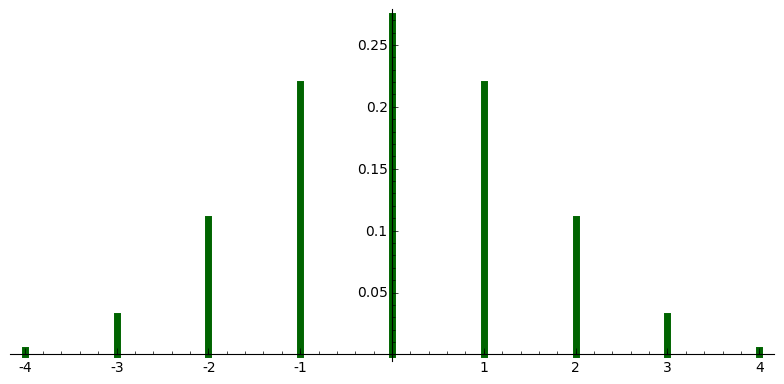
\includegraphics[width = 0.5\textwidth]{v8.png}
\caption{Probability density function of $\cV_{8}$}
\end{figure}


\begin{Definition}
\label{def: modified distribution}
Let $k \geq 2$ be an even integer. Then a sample from the modified PLWE error distribtuion $P'_{m,k}$ is
\[
    e' = \sum_{i=0}^{n-1} e'_i \zeta_m^{i},
\]
where the coefficients $e'_i$ are sampled independently from $\cV_k$.
\end{Definition}




\subsection{Fourier analysis}
We recall the definition and key properties of Fourier transform over finite fields.
Suppose $f$ is a real-valued function on $\bF_q$. The {\it Fourier transform} of $f$ is defined as
\[
    \widehat{f}(y) = \sum_{a \in \bF_q} f(a) \bar{\chi_y}(a),
\]
where $\chi_y(a) := e^{2 \pi i ay/q}$.

Let $u$ denote the probability density function of the uniform distribution over $\bF_q$, that is $u(a) = \frac{1}{q}$ for all $a \in \bF_q$. Let $\delta$ denote the characteristic function of the
one-point set $\{0\} \subseteq \bF_q$. Recall that the convolution of two functions $f,g$ is
\[
    (f  \ast g ) (a) = \sum_{b \in \bF_q} f(a-b)g(b).
\]
\begin{Fact}[Properties of Fourier transform] \label{fact: basicfourier}\qquad
\begin{enumerate}
\item $\widehat{\delta} = qu$.

\item  $\widehat{u} = \delta$.

\item $\widehat{f \ast g} = \widehat{f} \cdot \widehat{g}$.


\item $f(a) = \frac{1}{q} \sum_{y \in \bF_q} \widehat{f}(y)\chi_y(a)$.
%\item Plancherel's formula states that
%$||f||_2 = \frac{1}{q} ||\widehat{f}||_2$.

%\item $\widehat{f(a - \lambda)}(s) =  \bar{\chi_s(\lambda)} f(s)$.
\end{enumerate}
\end{Fact}

Suppose $f,g$ are the probability density functions of two random variables $F,G$ with value in $\bF_q$. Let $h$ denote the density function of the sum $H =F+G$.

\begin{Lemma}
Suppose the random variables $F,G$ are independent, then $h =  f \ast g$.
In general, suppose $F_1, \cdots, F_n$ are mutually independent random variables in $\bF_q$, with probability density functions $f_1, \cdots, f_n$. Let $f$ denote the density function of the sum $F = \sum F_i$, then $f = f_1 \ast \cdots \ast f_n$.
\end{Lemma}

\begin{proof}
We prove the first claim. For any $a \in \bF_q$,
\begin{align*}
\prob(F+G = a) &= \sum_{b \in \bF_q} \prob(F = a-b, G =b) \\
& = \sum_{b \in \bF_q} \prob(F = a-b)\prob(G =b).  \qquad \mbox{(since $F,G$ are independent)} \\
& = (f \ast g)(a).
\end{align*}
The general case follows from an induction on $n$.
\end{proof}

The Fourier transform of $\nu_k$ has a nice closed-form formula.
\begin{Lemma}
\label{lem: transform1}
For all even integers $k \geq 2$, $\widehat{\nu_k}(y)  = \cos \left(\frac{\pi y}{q}\right)^k.$
\end{Lemma}

\begin{proof}  We have
\begin{align*}
2^k \cdot \widehat{\nu_k}(y) &= \sum_{m = -\frac{k}{2}}^{\frac{k}{2}} {k \choose m+\frac{k}{2}} e^{2\pi i ym/q}  \\
&= e^{-\pi i yk/q}\sum_{m = -\frac{k}{2}}^{\frac{k}{2}} {k \choose m+\frac{k}{2}} e^{2\pi i y(m+k/2)/q} \\
&= e^{-\pi i yk/q} \sum_{m' = 0}^{k} {k \choose m'} e^{2\pi i ym'/q} \\
& =  e^{-\pi i yk/q} (1+ e^{2 \pi i y/q})^k \\
& = (e^{-\pi i y/q} + e^{\pi i y/q})^k  \\
& = (2 \cos(\pi y/q))^k.
\end{align*}
Dividing both sides by $2^k$ gives the result.
\end{proof}


Next, we concentrate on the reduced distributions $P_{m,\tau} \pmod{\fq}$ and $P'_{m,k} \pmod {\fq}$. Note that there is a one-to-one correspondence between primitive $m$-th roots of unity in $\bF_q$ and the prime ideals above $q$ in $\bQ(\zeta_m)$. Let $\alpha$ be the root corresponding to our choice of $\fq$. Then a sample from $P_{m, \tau} \pmod{\fq}$ (resp. $P'_{m,k} \pmod {\fq}$) is


$$ \sum_{i=0}^{n-1} \alpha^i e_i \pmod {q},$$

where $e_i$ are independent variables under the distribution $D_{\bZ,\tau}$ (resp. $\cV_k$). We use $e_\alpha$ and $e_\alpha'$ to denote their probability density functions. Then

\begin{Lemma}
\label{lem: transform2}
\[
    \widehat{e_\alpha'}(y) = \prod_{i=1}^{n} \cos \left(\frac{ \alpha^i \pi y}{q} \right)^k.
\]
\end{Lemma}

\begin{proof}
This follows directly from Lemma~\ref{lem: transform1} and Lemma~\ref{fact: basicfourier}.
\end{proof}

Now we are able to bound the difference  using the Fourier inversion formula.

\begin{Prop} \label{prop: bound}
Let $f: \bF_q \to \bR$ be a function such that $\sum_{a \in \bF_q} f(a) = 1$. Then for all $a \in \bF_q$,
\begin{equation} \label{eq: secure}
    |f(a) -  1/q| \leq \frac{1}{q}  \sum_{y \in \bF_q, y \neq 0}  |\hat{f}(y)|.
\end{equation}
\end{Prop}

\begin{proof} For all $a \in \bF_q$,
\begin{align*}
    f(a) - 1/q &= f - u(a) \\
    & = \frac{1}{q} \sum_{y \in \bF_q} (\hat{f}(y) - \widehat{u}(y) )\chi_y(a) \\
& = \frac{1}{q} \sum_{y \in \bF_q} (\hat{f}(y)  - \delta(y) )\chi_y(a) \\
& = \frac{1}{q} \sum_{y \in \bF_q, y \neq 0} \hat{f}(y)  \chi_y(a).  \qquad \mbox{(since $\hat{f}(0) = 1$)}
\end{align*}
Now the result follows from taking absolute values on both sides, and noting that $|\chi_y(a)| \leq 1$ for all $a$ and all $y$.
\end{proof}

Taking $f = e_\alpha$ or $f = e_\alpha'$ in Proposition~\ref{prop: bound}, we immediately obtain
\begin{theorem} \label{cor: stat dist}
The statistical distance between $e_\alpha$ and $u$ satisfies $$d(e_\alpha,u) \leq \frac{1}{2}  \sum_{y \in \bF_q, y \neq 0}  |\widehat{e_\alpha}(y)|.$$
Similarly,
\begin{equation} \label{distance}
d(e_\alpha',u) \leq \frac{1}{2}  \sum_{y \in \bF_q, y \neq 0}  |\widehat{e'_\alpha}(y)|.
\end{equation}
\end{theorem}



Now let $\epsilon'(m,q,k,\alpha)$ denote the right hand side of (\ref{distance}), i.e.,
\[
    \epsilon'(m,q,k, \alpha) = \frac{1}{2}\sum_{y \in \bF_q, y \neq 0} \prod_{i=0}^{n-1} \cos \left(\frac{ \alpha^i \pi y}{q} \right)^k.
\]
To take into account all prime ideals above $q$, we let $\alpha$ run through all primitive $m$-th root of unities in $\bF_q$ and define
$$\epsilon'(m,q,k) := \max \{\epsilon'(m,q,k,\alpha): \alpha \mbox{ has order } m \mbox{ in } \bF_q\}.$$
If $\epsilon'(m,q,k)$ is negligibly small, the distribution $P'_{m,k} \pmod {\fq}$ will be computationally indistinguishable from uniform. We have computed $\epsilon'(m,q,k)$ for various choices of parameters. The following is a table of data.


\begin{table}[H]
\label{tab: deg1}
\caption{Values of $\epsilon'(m,q,2)$}
\begin{tabular}{c|c|c|c}
$m$ & $n$ & $q$ & $-[\log_2(\epsilon'(m,q, 2))]$ \\
\hline
96 & 32 & 4513 & $35$ \\
55 & 40 & 10891  & $44$ \\
160 & 64 &20641 & 61 \\
101 & 100 & 1213 & $177$ \\
145 & 112  &19163 & $176$ \\
244 & 120 & 1709 & 230 \\
256 & 128 & 3329 & $194$ \\
256 & 128 & 14081 & $208$ \\
197 & 196 & 3547 & $337$ \\
512 & 256 &10753 & 431 \\
512 & 256 &19457 & 414
\end{tabular}
\end{table}

The data in Table~\ref{tab: deg1} suggests that for $n \geq 100$ and $q$ polynomial in $n$, the statistcal distance between $P'_{m,k} \pmod{\fq}$ and the uniform distribution is negligibly small. As a consequence, any attack that reduce the errors modulo $\fq$ will be unlikely to succeed. Note that we fixed $k= 2$, and $\epsilon'(m,q,k)$ decreases with $k$.

We can run the same analysis for the PLWE distributio, with the only difference being that there is no obvious closed-form formula for the density function $d$  of $D_{\bZ,\tau} \pmod{q}$. Nonetheless, we could numerically approximate this probability density function, using the formula
\[
  d(a)  = \frac{\sum_{z \in \bZ, z \equiv a\pmod{q}} e^{-|z|^2/2\tau}}{\sum_{z \in \bZ} e^{-|z|^2/2\tau}}, \quad \forall a \in \bF_q.
\]
Since the sums in the definition of $d(a)$ converge rapidly, we could obtain good approximations of $d$ by truncating the sums. Then we compute its Fourier transform $\hat{d}$, and obtain
\[
    \widehat{e_\alpha}(y) = \prod_{i=0}^{n-1} \hat{d}(\alpha^i y)
\]
Finally, we can compute $\epsilon(m,q,\tau) = \frac{1}{2} \sum_{y \in \bF_q, y \neq 0} \prod_{i=0}^{n-1} \widehat{d}(\alpha^i y)$. Then $\epsilon(m,q,\tau)$ is an upper bound of the statistical distance  between the distribution $e_\alpha$ and the uniform distribution over $\bF_q$. Table~\ref{table: deg2} contains some data for values of $\epsilon(m,q,\tau)$.



\FloatBarrier
\begin{table}[H]
\label{table: deg2}
\caption{Values of $\epsilon(m,q,\tau)$}
\begin{tabular}{c|c|c|c}
$m$ & $n$ & $q$ &  $-[\log_2(\epsilon(m,q, 1))]$ \\
\hline
96 & 32 & 4513 & $35$ \\
55 & 40 & 10891  & $44$ \\
160 & 64 &20641 & 61 \\
101 & 100 & 1213 & 203 \\
145 & 112  &19163 & $176$ \\
244 & 120 & 1709 & 247 \\
256 & 128 & 3329 & 252\\
256 & 128 & 14081 & $208$ \\
197 & 196 & 3547 & $337$ \\
512 & 256 &10753 & 431 \\
512 & 256 &19457 & 414
\end{tabular}
\end{table}


\begin{remark}
It is possible to generalize our discussion in this section to higher degree primes, where the Fourier analysis is performed in extension fields $\bF_{q^f}$. The only change in the definition would be $\chi_y(a) = e^{ \frac{2 \pi i Tr(a_i y)}{q}}$, and we have
\[
    \widehat{e'_\alpha}(y) = \prod_{i=1}^{n} \cos \left(\frac{ \pi Tr(\alpha^i y) }{q} \right)^k.
\]
Table~\ref{tab: deg2} contains some data for primes of degree two.
\end{remark}

\FloatBarrier
\begin{table}[H] \label{tab: deg2}
\caption{Values of $\epsilon'(m,q,2)$ for primes of degree 2}
\begin{tabular}{c|c|c}
$m$ & $q$ & $-[\log_2(\epsilon'(m,q,2))]$ \\
\hline
53 & 211 & 61 \\
55 & 109 & 48 \\
63 & 881 & 33 \\
%64 & 127 & 37 \\
%64 & 191 & 35 \\
64 & 383 & 31 \\
512 & 257 & 263
\end{tabular}
\end{table}

\begin{remark}
There is a heuristic argument on why one expects $\epsilon'(m,q,k,\alpha)$ to be small. Each term in the summand is a product of cosines of form $\prod_{i=0}^{n-1} \cos \left(\frac{ \alpha^i \pi y}{q} \right)^k$. For each $0 \neq y \in \bF_q$, Since the elements $\alpha^i$ are distinct and usually spaced-out in $\bF_q$, it is very likely that $\alpha^i y$ is close $q/2$ for some values of $i$, making the product of cosines small.
\end{remark}

\bibliographystyle{amsalpha}
\bibliography{galois-rlwe}

\end{document}
